\documentclass{article}

\usepackage{graphicx}
\usepackage{amsmath}
\usepackage{float}

\title{Autoencoder Bottleneck Compression Study}
\author{}
\date{}

\begin{document}

\maketitle

\section{Problem Definition}

Autoencoders are neural networks used for unsupervised representation learning. 
They compress input data into a lower-dimensional representation called a \textbf{latent space} 
and then reconstruct the original input.

The objective of this experiment is to investigate how the size of the latent bottleneck affects 
reconstruction quality when compressing handwritten digit images from the MNIST dataset.

\section{Architecture}

The implemented symmetric autoencoder consists of the following structure.

\textbf{Encoder}

\[
784 \rightarrow 128 \rightarrow 64 \rightarrow N
\]

\textbf{Decoder}

\[
N \rightarrow 64 \rightarrow 128 \rightarrow 784
\]

Where \(N\) represents the latent bottleneck dimension.

Two experiments were performed:

\begin{itemize}
\item Bottleneck size \(N = 2\)
\item Bottleneck size \(N = 32\)
\end{itemize}

\section{Methodology}

\begin{itemize}
\item Dataset: MNIST handwritten digits
\item Input Size: \(28\times28\) grayscale images
\item Flattened Input Vector: 784
\item Loss Function: Mean Squared Error (MSE)
\item Optimizer: Adam
\item Learning Rate: 0.001
\item Epochs: 10
\item Batch Size: 128
\end{itemize}

Each image was flattened into a vector of size \(784\) before being passed to the network.

\section{Results}

The quality of reconstruction was analyzed visually by comparing original images with reconstructed images.

\subsection{Latent Space Visualization (N = 2)}

\begin{figure}[H]
\centering
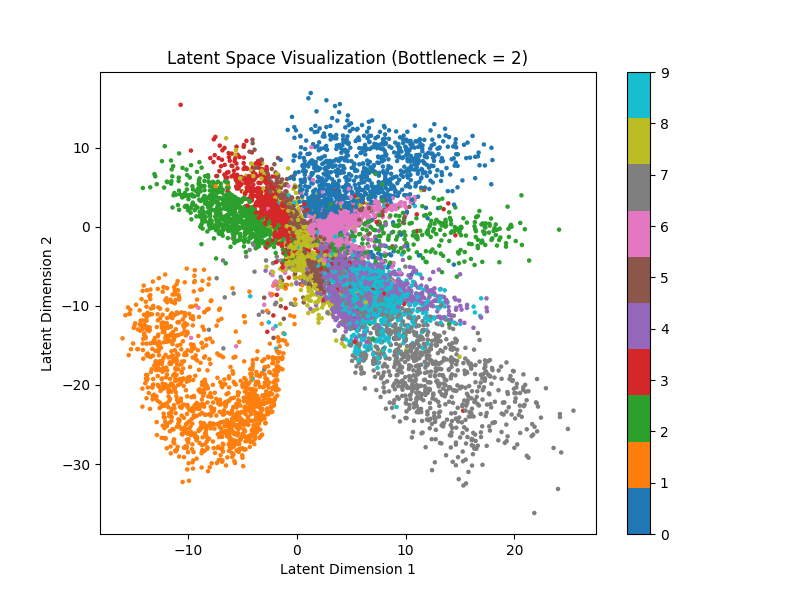
\includegraphics[width=0.8\linewidth]{plots/bottleneck_2_latent.png}
\caption{2D latent representation learned by the autoencoder with bottleneck size 2. Each point corresponds to a digit encoded into the two-dimensional latent space.}
\end{figure}

This visualization shows how the encoder organizes digit images into a compressed two-dimensional space. 
Even though the model was trained without labels, similar digits tend to cluster together, indicating that 
the network has learned meaningful structural features of the digits.

\subsection{Latent Space Visualization (N = 32)}

\begin{figure}[H]
\centering
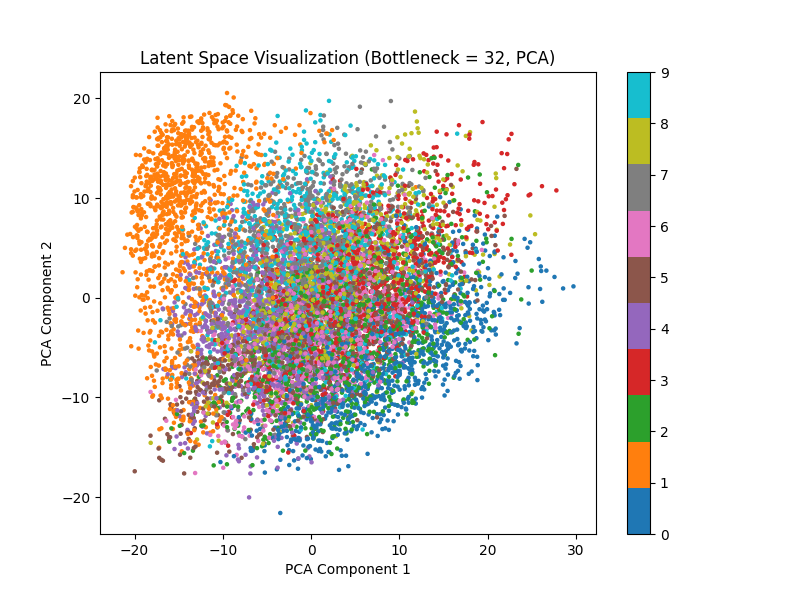
\includegraphics[width=0.8\linewidth]{plots/bottleneck_32_latent.png}
\caption{Latent representation for bottleneck size 32 projected to two dimensions using PCA.}
\end{figure}

Since the latent representation contains 32 dimensions, PCA was used to reduce it to two dimensions for visualization. 
The clusters appear more structured because the higher-dimensional latent space allows the network to encode more detailed information about each digit.

\subsection{Reconstruction with Bottleneck Size \(N = 2\)}

\begin{figure}[H]
\centering
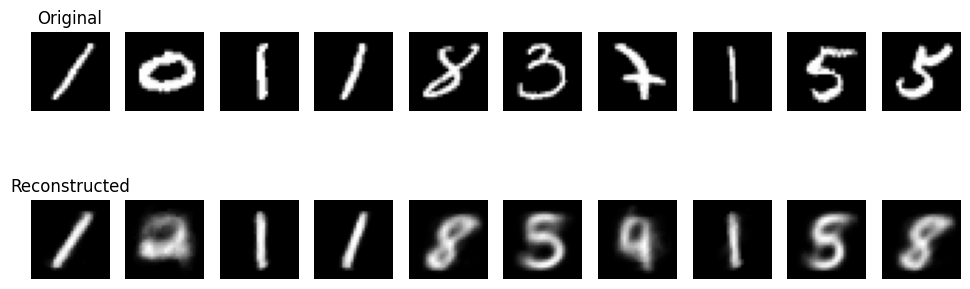
\includegraphics[width=0.9\linewidth]{plots/bottleneck_2.png}
\caption{Original vs reconstructed MNIST digits using a bottleneck size of 2.}
\end{figure}

With only two latent variables, the network compresses the entire image into an extremely small representation. 
As a result, the reconstructed images appear blurry and lose important structural details of the digits.

\subsection{Reconstruction with Bottleneck Size \(N = 32\)}

\begin{figure}[H]
\centering
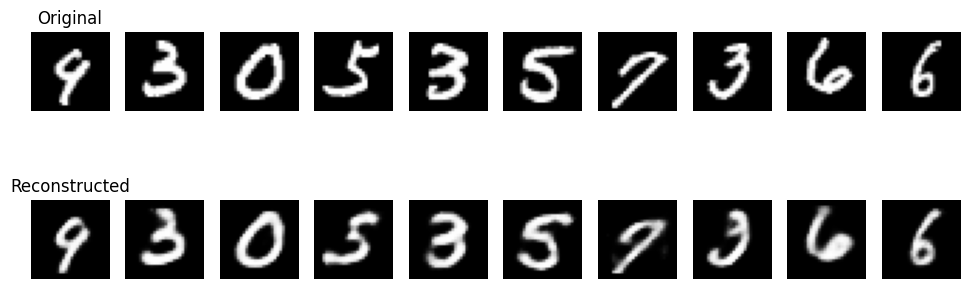
\includegraphics[width=0.9\linewidth]{plots/bottleneck_32.png}
\caption{Original vs reconstructed MNIST digits using a bottleneck size of 32.}
\end{figure}

With a larger latent space, the network can preserve significantly more information about the input image. 
This leads to clearer reconstructions and better preservation of digit structure.

\section{Key Findings}

\begin{itemize}
\item The latent bottleneck dimension strongly affects reconstruction quality.
\item Extremely small bottlenecks force aggressive compression and cause information loss.
\item Larger latent spaces allow the model to encode more meaningful features.
\item Autoencoders learn compact representations while balancing compression and reconstruction accuracy.
\end{itemize}

\section{Conclusion}

This experiment demonstrates the importance of latent space dimensionality in autoencoder architectures. 
A very small bottleneck forces the model to learn only the most dominant features, resulting in degraded reconstructions. 
Increasing the bottleneck size allows the model to preserve more information, producing higher quality reconstructions.

\end{document}